% Homework report template for courses lectured by Blaz Zupan.
% For more on LaTeX please consult its documentation pages, or
% read tutorials like http://tobi.oetiker.ch/lshort/lshort.pdf.
%
% Use pdflatex to produce a PDF of a report.

\documentclass[a4paper,10pt]{paper}
\usepackage[utf8]{inputenc}
\usepackage{a4wide}
\usepackage{fullpage}
\usepackage{caption}
\usepackage{subcaption}
\usepackage{float}
\usepackage{amsmath}
\usepackage{amsfonts}
\usepackage{amssymb}

\usepackage[toc,page]{appendix}
\usepackage[pdftex]{graphicx} % for figures
\usepackage{setspace}
\usepackage{color}
\definecolor{light-gray}{gray}{0.95}
\usepackage{listings} % for inclusion of Python code
\usepackage{hyperref}
\renewcommand{\baselinestretch}{1.2}
\def\code#1{\texttt{#1}}
\lstset{ % style for Python code, improve if needed
language=Python,
basicstyle=\footnotesize,
basicstyle=\ttfamily\footnotesize\setstretch{1},
backgroundcolor=\color{light-gray},
}

\usepackage{titling}
\usepackage{blindtext}
 
\setlength{\droptitle}{-7em}     % Eliminate the default vertical space
\addtolength{\droptitle}{-18pt}   % Only a guess. Use this for adjustment


\title{Seminarska naloga 1 - Spletni pajek\\\vspace{-1em}}
\author{Andraž Jelenc, Vid Križnar, Sandi Režonja}

\begin{document}

\maketitle
\vspace{-3em}

\section{Uvod}
Cilj seminarske naloge je bila izdelava pajka za preiskovanje spletišč domene gov.si. Pajek deluje po principu iskanja v širino in implementira vzporedno delovanje več pajkov.
Napisan je v jeziku Python, za podatkovno bazo smo izbrali PostgreSQL 9. Oba tečeta vsak v svojem Docker kontejnerju. Nastavitve pajka, kot so začetne strani in število vzporednih pajkov, nastavimo v datoteki docker-compose.yml. Vse skupaj pa nato zaženemo z uporabo orodja Docker Compose.
\section{Implementacija}


\subsection{Frontier}
Frontier smo implementirali v bazi s tabelo \code{crawldb.page}. Sestavljajo ga tiste strani, katerih \code{page\_type} atribut je bil nastavljen na FRONTIER. Spoštovanje zakasnitve smo implementirali z razširitvijo baze s tabelo \code{crawldb.server}, v katero smo shranili IP naslov strežnika in čas zadnjega obiska. Tabelo \code{crawldb.site} smo razširili s poljem želenega premora med obiski. Iskanje naslednje strani za obdelavo je iz fontierja vrnilo stran z najmanjšim indeksom, ki je zadoščala zakasnitvenem pogoju.

Pri dodajanju, pajek preskoči strani, ki niso iz domene gov.si. Če strežnika še ne pozna, najprej tega doda v bazo. Če ne pozna domene, doda novo in pri tem prenese vsebino strani robots.txt, poveča zakasnitveni pogoj, če je to zahtevano in poskusi najdi sitemap datoteko. Če le-ta obstaja, shrani pot do datoteke v bazo, vse URL naslove, ki jih le-ta vsebuje pa doda v frontier. Nato nadaljuje z dodajanjem trenutne strani. Če domena premore sitamap, robots.txt prepoveduje obisk strani ali pa je stran že v frontierju, je ne doda. Če smo dodali novo stran, ustvarimo nov vnos za povezavo med novo stranjo in stranjo, kjer smo našli ta URL naslov.

\subsection{Vzporednost}
Delovanje več vzporednih pajkov smo zagotovili z večnitnostjo. Vsak pajek je deloval do izpolnitve zaustavitvenega pogoja – praznega frontierja. Vendar se zaradi več vzporednih pajkov lahko zgodi, da je frontier prazen le začasno. Zato pajek frontier večkrat preveri in se ustavi šele po določenem številu poskusov. Ko pajek iz frontierja prenese URL naslov naslednje strani, pri tem posodobi zadnji čas dostopa do strežnika in nastavi status strani na PROCESSING. Nato začne z obdelavo strani.

\subsection{Obdelava}
S selenium-wire (razširitev ogrodja Selenium) prenesemo vsebino strani, na katero kaže izbrani URL. Prenašanju velikih binarnih datotek se izognemo tako, da omejimo čas prenosa. Če je časovna omejitev presežena, strani nastavimo status \code{null}, s čim zabeležimo napako. Med nalaganjem sledimo preusmeritvam in vrnemo status in tip vsebine prvega odgovora, ki nas ne preusmerja drugam, če tak odgovor obstaja. Če status odgovora ni enak statusu 200 OK, v podatkovno bazo shranimo le tip vsebine in status, s samo vsebino pa se ne ukvarjamo. Sicer pa obravnavo ločimo na dva primera. Če gre za binarno datoteko nastavimo tip strani na BINARY in v primeru, da gre za PDF, DOC, DOCX, PPT ali PPTX datoteko v tabeli \code{page\_data} dodamo zapis o najdenem dokumentu. Vsebine binarne datoteke ne shranjujemo. V primeru HTML strani pa preverimo, ali MD5 vrednost vsebine že poznamo (duplikat), nato pa iz vsebine izluščimo vse URL naslove iz atributov \code{href} in \code{onclick}. Pred dodajanjem najdenih naslovov v frontier, relativne naslove pretvorimo v absolutne in nad naslovi izvedemo kanonizacijo, poleg tega naslovom odstranimo začetne \code{www}. Iz vsebine izluščimo tudi vse \code{src} atribute slik na strani. Za vsako sliko dodamo zapis v \code{crawldb.image}, kjer poleg naslova datoteke poskusimo iz njega izluščiti še tip slike.



\section{Rezultati}
Pajka smo pustili teči 82 ur, pri tem smo uporabili 4 niti. V tem času je preiskal povprečno 3 domene na uro in pri tem obdelal 886 strani na uro. Natančnejši podatki so na voljo v tabeli \ref{table:tab1}. Število vseh strani, ki jih zaradi različnih razlogov nismo uspeli prenesti v celoti (neodzivnost strežnika, časovni limit...) je navedeno v vrstici \# z napako.
Z orodjem Gephi smo vizualizirali povezanost med domenami. Na vizualizaciji \ref{vv} je prikazana povezanost domen, med katerimi je vsaj 50 linkov med spletnimi stranmi. Velikost imena domene predstavlja število strani, velikost povezave pa število linkov. Oboje je v logaritemski skali. Izvoz baze je zaradi velikosti naložen na Dropbox, na Github pa smo objavili le link.
 \begin{table}[H]

\begin{tabular}{|l|l|l|l|l|l|}

\hline

                     & (vse domene) & gov.si & evem.gov.si & e-uprava.gov.si & e-prostor.gov.si \\ \hline

\# domen             & 247          & -      & -           & -               & -                \\ \hline

\# strani / domeno   & 294         & -      & -           & -               & -                \\ \hline

\# vseh strani       & 72683        & 24369  & 6443        & 20939           & 516              \\ \hline

\# html strani       & 49105        & 20751  & 3937        & 17454           & 166              \\ \hline

\# duplikatov        & 372          & 132    & 35          & 0               & 10               \\ \hline

\# DOC               & 436          & 0      & 31          & 146             & 27               \\ \hline

\# DOCX              & 257          & 0      & 0           & 91              & 3                \\ \hline

\# PDF               & 1052         & 0      & 102         & 189             & 112              \\ \hline

\# PPT               & 1            & 0      & 0           & 0               & 1                \\ \hline

\# PPTX              & 1            & 0      & 0           & 0               & 0                \\ \hline

\# druge binarne     & 592          & 3      & 90          & 42              & 86               \\ \hline

\# slik              & 100229       & 28148  & 19535       & 17684           & 60               \\ \hline

\# slik / html stran & 2,0          & 1,4    & 5,0         & 1,0             & 0,4              \\ \hline

\# z napako          & 20867        & 3483   & 2248        & 3017            & 111              \\ \hline

\end{tabular}
\caption{Statistični podatki pajkovega delovanja.}
\label{table:tab1}
\end{table}


\begin{figure}[H]
\hspace*{-1cm}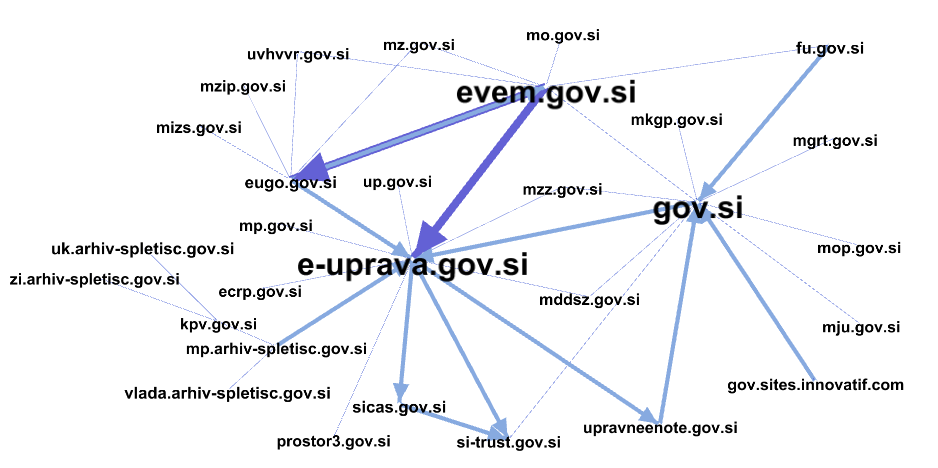
\includegraphics[width=14cm]{graf.png}
\centering

\caption{Vizualizacija povezanosti domen.}
\label{vv}
\end{figure}


\section{Literatura}
\begin{itemize}
  \item https://gephi.org
  \item https://docs.python.org/3/library/threading.html
  \item https://pypi.org/project/psycopg2/
  \item https://pypi.org/project/selenium-wire/
\end{itemize}



\end{document}
